\documentclass[11pt]{amsbook}

\usepackage{../HBSuerDemir}	% ------------------------


\begin{document}

% ++++++++++++++++++++++++++++++++++++++
\hPage{b2p1/122}
% ++++++++++++++++++++++++++++++++++++++



% =======================================
    \[ \left| C \right| = \sqrt[]{(\frac{1}{9})^2 + (\frac{4}{9})^2 + (\frac{8}{9})^2 } = \frac{1}{9} \sqrt[]{1 + 16 + 64} = 1 \]
    
    
    \\ A vector having lenth equal to 1 is called a \underline{unit vector}. In the above example, C is seen to be a unit vector.
    
    
% =======================================


    \subsection*{\underline{B. ALGEBRA OF VECTORS}}~
    
    \\1. \underline{Addition}:
    \\ The sum \(\vec{a} + \vec{b}\) of two vectors \(\vec{a}\) and \(\vec{b}\), in this order, is the vector whose initial point is that of the first and the extremity is that of the second when the latter is translated to have its initial point at the extremity of the first vector:
    \\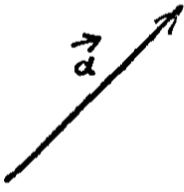
\includegraphics[scale = 0.7]{images/b2p1-122_fig1} 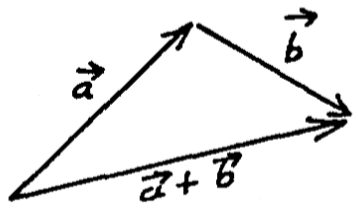
\includegraphics[scale=0.7]{images/b2p1-122_fig2}
    
    \\ The following figures are the commutative law 
     \[ \vec{a} + \vec{b} =  \vec{b} + \vec{a}\]
    \\ and the parallelogram law:
    \\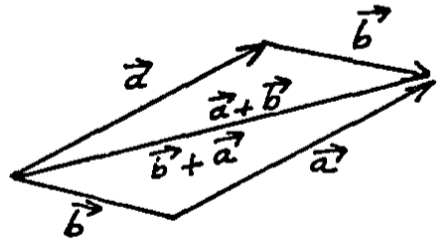
\includegraphics[scale=0.7]{images/b2p1-122_fig3}
    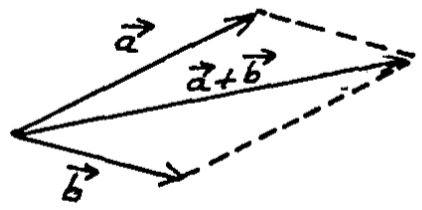
\includegraphics[scale = 0.7]{images/b2p1-122_fig4}
    
    \\ The associative law
     \[ (\vec{a} + \vec{b}) + \vec{c} =  \vec{a} + (\vec{b} + \vec{c})\]
     \\ is the result congruency of the following pyramids:
      \\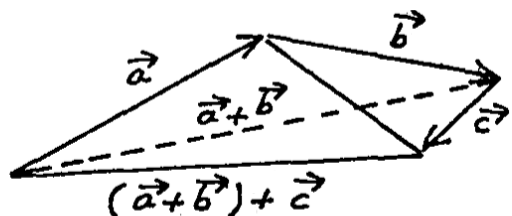
\includegraphics[scale=0.7]{images/b2p1-122_fig5}
      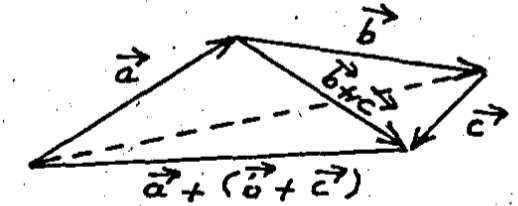
\includegraphics[scale = 0.7]{images/b2p1-122_fig6}
      
      \\ Because of this law the sum \( \vec{a} + \vec{b} + \vec{c} \) has a meaning as defined by \( (\vec{a} + \vec{b}) + \vec{c} \) or by \( \vec{a} + (\vec{b} + \vec{c}) \)
    
    
   
% =======================================
  

% =======================================================
\end{document}  

%==== templates ====

%==== environments ====

%\begin{figure}[htb]
%	\centering
%	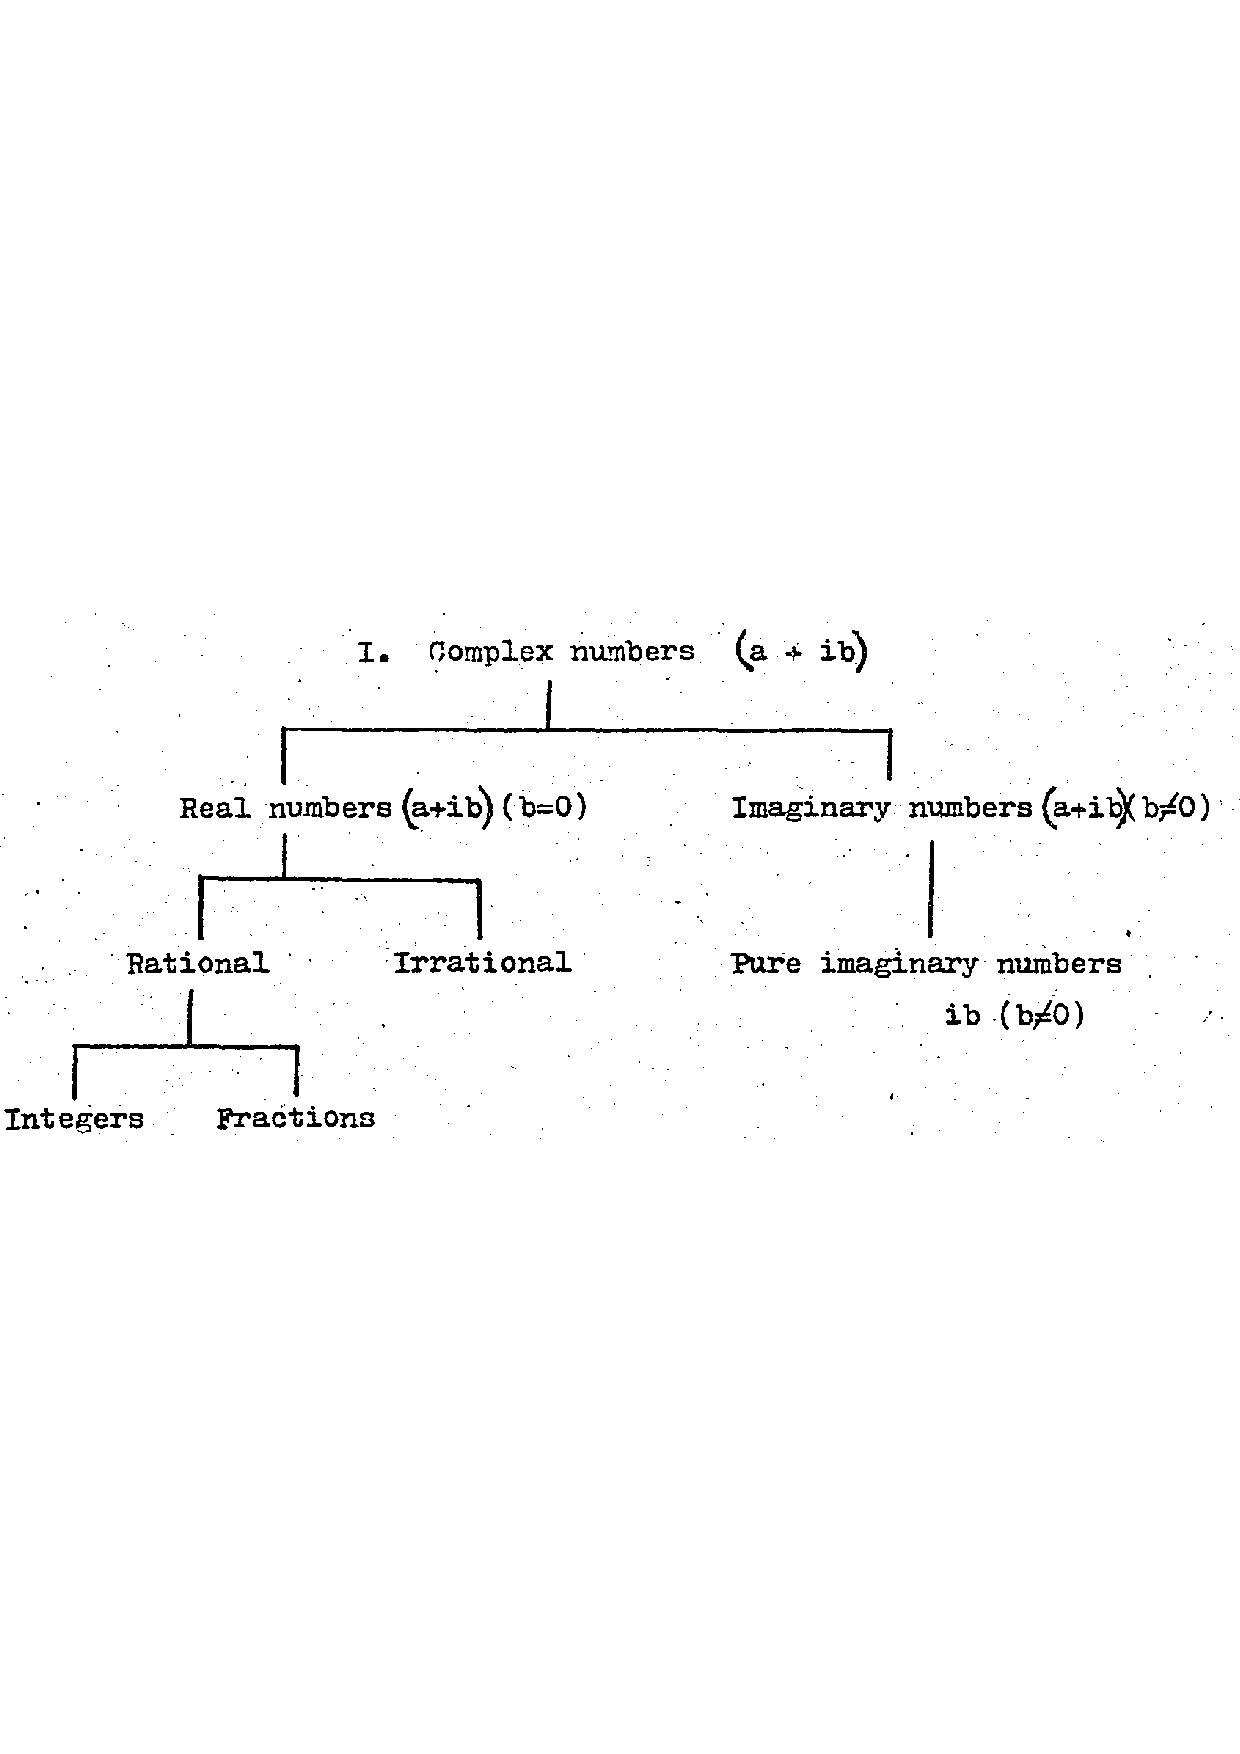
\includegraphics[width=0.9\textwidth]{images/SD-1-1p15A}
%	\caption{Classification of complex numbers}
%	\label{fig:classificationOfComplexNumbersA}
%\end{figure}

%\begin{center}
%\begin{tabular}{cc}
%\end{tabular}
%\end{center}

%\begin{exmp}
%\begin{hSolution}
%\end{hSolution}
%\end{exmp}

%\begin{hEnumerateAlpha}
%\end{hEnumerateAlpha}

%\begin{hEnumerateRoman}
%\end{hEnumerateRoman}

%$
%\begin{bmatrix}
%\end{bmatrix}
%$

%\frac{aaaa}{bbb}
%\frac{a_{n}}{b_{n}}
%\left( aaaa \right)
%\Longrightarrow

%\begin{multicols}{2}
%	bb
%\columnbreak
%	aa
%\end{multicols}
